\documentclass[conference]{IEEEtran}
\usepackage{newtxtext,newtxmath}
\usepackage{graphicx,booktabs,amsmath,url,cite,xcolor,array}
\usepackage[hidelinks]{hyperref}

% ======================= EDIT TEAM DETAILS HERE ============================
\newcommand{\MemA}{Tathagat Harsh}  \newcommand{\RollA}{2401010477}
\newcommand{\MemB}{M S Thejas}  \newcommand{\RollB}{2401010255}
\newcommand{\MemC}{Garv Verma}  \newcommand{\RollC}{2401010168}
\newcommand{\MemD}{Parv Goyal}  \newcommand{\RollD}{2401010322}
\newcommand{\MemE}{Vaibhav Rajput}  \newcommand{\RollE}{2401010487}
\newcommand{\RepoURL}{https://github.com/TathagatHarsh/dm-cache-controller}
\newcommand{\VideoURL}{https://drive.google.com/drive/folders/1XrK8QC8PR5nWN_Udr-LCHOQUd5ePlpkO?usp=sharing}
% ============================================================================

\begin{document}
\title{Design and Verification of a Direct-Mapped Cache Controller in Verilog HDL\\
{\large Phase I Report --- CSA222 Modern Computer Architecture (Project 6)}}

\author{
\IEEEauthorblockN{\MemA, \MemB, \MemC, \MemD, \MemE}
\IEEEauthorblockA{\RollA, \RollB, \RollC, \RollD, \RollE\\
B.Tech (CS\&AI), Rishihood University / Newton School of Technology}}

\maketitle

\begin{abstract}
Processor speed has grown much faster than main-memory (DRAM) latency, so modern processors depend on small, fast SRAM caches that exploit program locality. This report presents the design and functional verification of a direct-mapped cache controller written in synthesizable Verilog HDL. The cache holds 1\,KB of data in 64 lines of 16-byte blocks and uses 32-bit byte addresses split into a 22-bit tag, 6-bit index and 4-bit offset. It follows a write-through, no-write-allocate policy. The design is split into seven modules: address decoder, tag RAM, valid-bit RAM, data RAM, tag comparator, a four-state controller FSM, and a main-memory model with configurable latency. Built-in hardware counters record hits and misses. A self-checking testbench with a golden reference model checks every access, both its hit/miss result and its data, across six traces (2{,}187 accesses), with zero mismatches. Hit rates range from 0\% for a conflict trace to 93.75\% for a loop trace. The measured average memory access time (AMAT) matches the analytical value $1 + m \times 11$ cycles on every trace. These results confirm the controller and demonstrate the effects of spatial locality, temporal locality and conflict misses in a direct-mapped cache.
\end{abstract}

\begin{IEEEkeywords}
cache memory, direct-mapped cache, cache controller, finite state machine, AMAT, Verilog, memory hierarchy
\end{IEEEkeywords}

\section{Introduction}
Main-memory latency (50--100\,ns for DRAM) is one to two orders of magnitude higher than a processor clock period. This growing gap is called the \emph{memory wall}~\cite{wulf1995}. Computer architects close the gap with a memory hierarchy: a small, fast SRAM cache sits between the processor and DRAM and holds recently used blocks~\cite{hp_coa,hp_caqa}. The idea works because real programs show \emph{temporal locality} (recently used data is reused soon) and \emph{spatial locality} (nearby addresses are used together).

A \emph{direct-mapped} cache is the simplest organization. Each memory block can live in exactly one cache line, chosen by the index bits of its address. This makes lookup a single tag comparison, with no replacement policy and no parallel ways, which gives a short hit time and low hardware cost~\cite{hill1988}. The price is \emph{conflict misses}: two frequently used blocks that share an index evict each other.

\textbf{Objective.} Following the course project specification (Project~6), we design a direct-mapped cache controller in Verilog, verify its lookup and refill behavior, and measure hit ratio, miss ratio and AMAT using sequential, repeated, random and conflicting memory-access traces.

\textbf{Phase I scope.} This report covers the complete RTL prototype, the controller FSM, a self-checking testbench, waveform evidence and preliminary hit-rate/AMAT results. Phase II will add FPGA synthesis (resource use and maximum frequency in Vivado), a comparison with a 2-way set-associative cache, and parameter sweeps.

\section{Literature Review}
\textbf{Origins.} Wilkes first proposed a small, fast ``slave memory'' that automatically holds copies of recently used main-memory words~\cite{wilkes1965}. This is the concept now called a cache. Smith's survey~\cite{smith1982} formalized the main design choices (placement, block size, fetch, replacement and write policy) and showed with trace-driven simulation that even small caches capture most references, because programs exhibit locality.

\textbf{Direct-mapped vs.\ associative.} Hill~\cite{hill1988} argued that direct-mapped caches can beat set-associative ones in \emph{effective} access time. Their hit path is shorter: no way-select multiplexer sits after the tag compare, and data can be forwarded speculatively before the hit is confirmed. This advantage grows as caches get larger, because the gain in miss ratio from associativity shrinks. Hill and Smith~\cite{hill1989} introduced the ``3C'' model, which classifies misses as compulsory, capacity and conflict. They quantified that associativity removes mainly conflict misses. The conflict trace in our work reproduces the worst case of this effect.

\textbf{Reducing conflict misses.} Jouppi~\cite{jouppi1990} kept the fast direct-mapped hit path and recovered most conflict misses by adding a small fully associative \emph{victim cache} and stream buffers for prefetching. Belady's study of replacement algorithms~\cite{belady1966} supplies the background for associative designs. A direct-mapped cache needs no such policy, because the victim is always fixed by the index.

\textbf{Write policies and controller design.} Patterson and Hennessy~\cite{hp_coa} describe a simple cache controller as a four-state FSM (Idle, Compare Tag, Write-Back, Allocate). They also compare write-through with write-back and write-allocate with no-write-allocate. Write-through keeps memory always consistent and needs no dirty bits, at the cost of more memory traffic, which is usually hidden by a write buffer~\cite{hp_caqa}. Our controller adapts this FSM to a write-through, no-write-allocate policy: the Write-Back state is replaced by a WRITE\_MEM state that forwards every store to memory. Hennessy and Patterson~\cite{hp_caqa} also define the performance metric we use, $\mathrm{AMAT} = t_{hit} + m \times t_{penalty}$.

\textbf{Gap addressed.} Textbooks present these ideas analytically. Our project turns them into verified hardware. We give a cycle-accurate RTL implementation in IEEE~1364 Verilog~\cite{verilog2005} together with hardware performance counters. A reference-model testbench lets us confirm the analytical hit-rate and AMAT predictions against measured cycle counts.

\section{Proposed Solution}
\subsection{Cache Parameters and Address Breakdown}
Table~\ref{tab:params} lists the configuration recommended by the project specification. All sizes are Verilog parameters, so they can be changed for the Phase~II parameter sweep.

\begin{table}[h]
\centering
\caption{Cache configuration}
\label{tab:params}
\begin{tabular}{@{}ll@{}}
\toprule
Parameter & Value \\ \midrule
Address width & 32 bits (byte addressed) \\
Cache data capacity & 1\,KB \\
Block (line) size & 16 bytes = 4 words \\
Number of lines & $1024/16 = 64$ \\
Offset / Index / Tag & 4 / 6 / 22 bits \\
Write policy & write-through, no-write-allocate \\
Main-memory latency $L$ & 10 cycles (parameter) \\
Hit time / miss penalty & 1 cycle / $L+1 = 11$ cycles \\ \bottomrule
\end{tabular}
\end{table}

The address decoder splits an address $A$ into
\[
\underbrace{A[31{:}10]}_{\text{tag (22)}}\;|\;\underbrace{A[9{:}4]}_{\text{index (6)}}\;|\;\underbrace{A[3{:}2]}_{\text{word}}\;|\;\underbrace{A[1{:}0]}_{\text{byte}}.
\]
The total storage is $64\times(128+22+1) = 9{,}664$ bits, of which 8{,}192 bits are data.

\subsection{Microarchitecture}
Fig.~\ref{fig:block} shows the datapath. The controller latches the CPU request into \texttt{addr\_q}. The decoder drives the index into the tag, valid and data RAMs, which all have asynchronous reads, and the comparator produces
$\textit{hit} = \textit{valid}[i] \wedge (\textit{tag\_ram}[i] = \textit{tag})$
in the same cycle. The valid bits sit in flip-flops so that a single reset clears all 64 lines; this prevents false hits on uninitialized tag RAM. On a read miss, the 128-bit block returned by memory is written to the cache. In the same cycle, the requested word is forwarded to the CPU through the word-select multiplexer, which saves one cycle compared with re-reading the cache.

\begin{figure}[t]
\centering
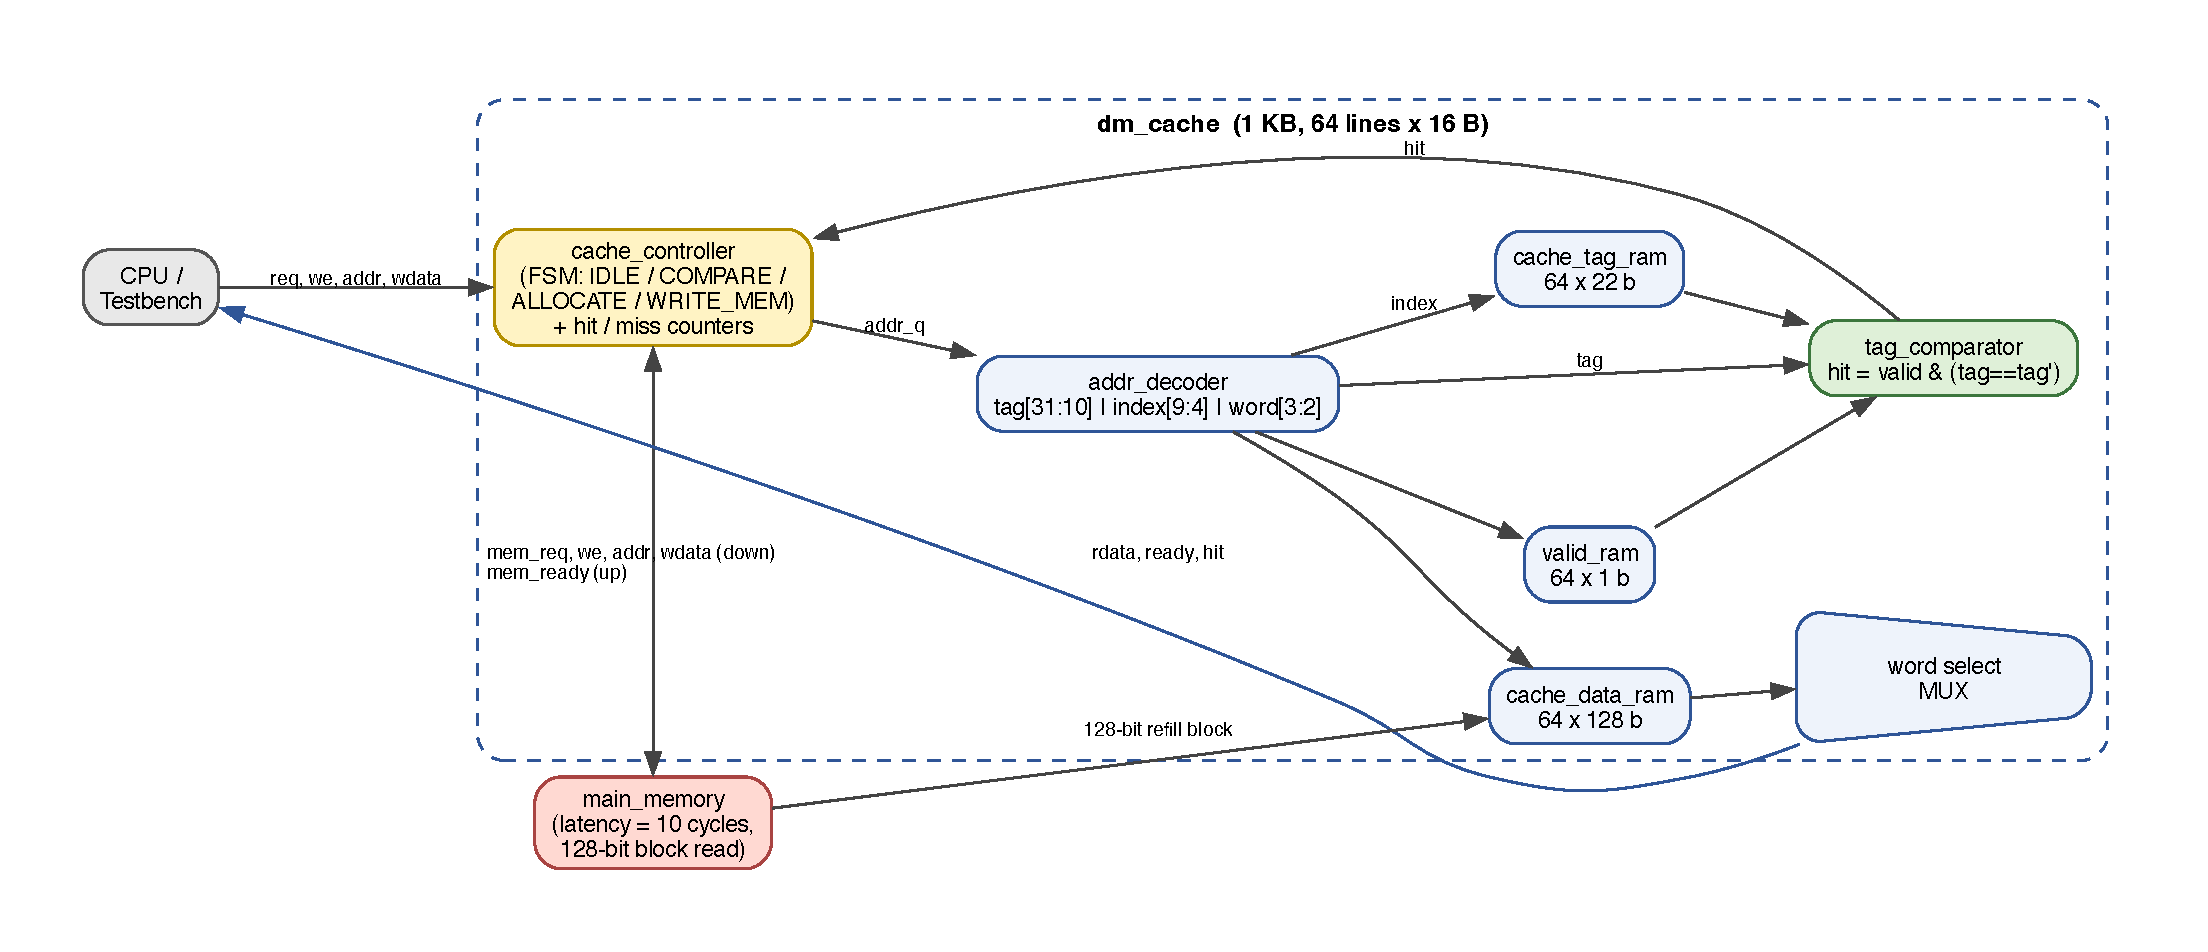
\includegraphics[width=\columnwidth]{../figures/block_diagram.pdf}
\caption{Block diagram of the direct-mapped cache and its interfaces.}
\label{fig:block}
\end{figure}

\subsection{Controller FSM}
The controller (Fig.~\ref{fig:fsm}) has four states:
\begin{itemize}
\item \textbf{IDLE}: waits for \texttt{cpu\_req} and latches address, data and the read/write flag.
\item \textbf{COMPARE}: checks the tag. A read hit returns data in this cycle (hit time = 1 cycle). A read miss goes to ALLOCATE. Any write goes to WRITE\_MEM, and a write hit also updates the cached word. The hit or miss counter is incremented here.
\item \textbf{ALLOCATE}: holds \texttt{mem\_req} until \texttt{mem\_ready}, then writes the block, tag and valid bit and completes the read.
\item \textbf{WRITE\_MEM}: forwards the store to memory (write-through). A write miss does not allocate a line.
\end{itemize}
The memory-interface outputs depend only on the state (Moore style). This keeps the memory handshake free of glitches.

\begin{figure}[t]
\centering
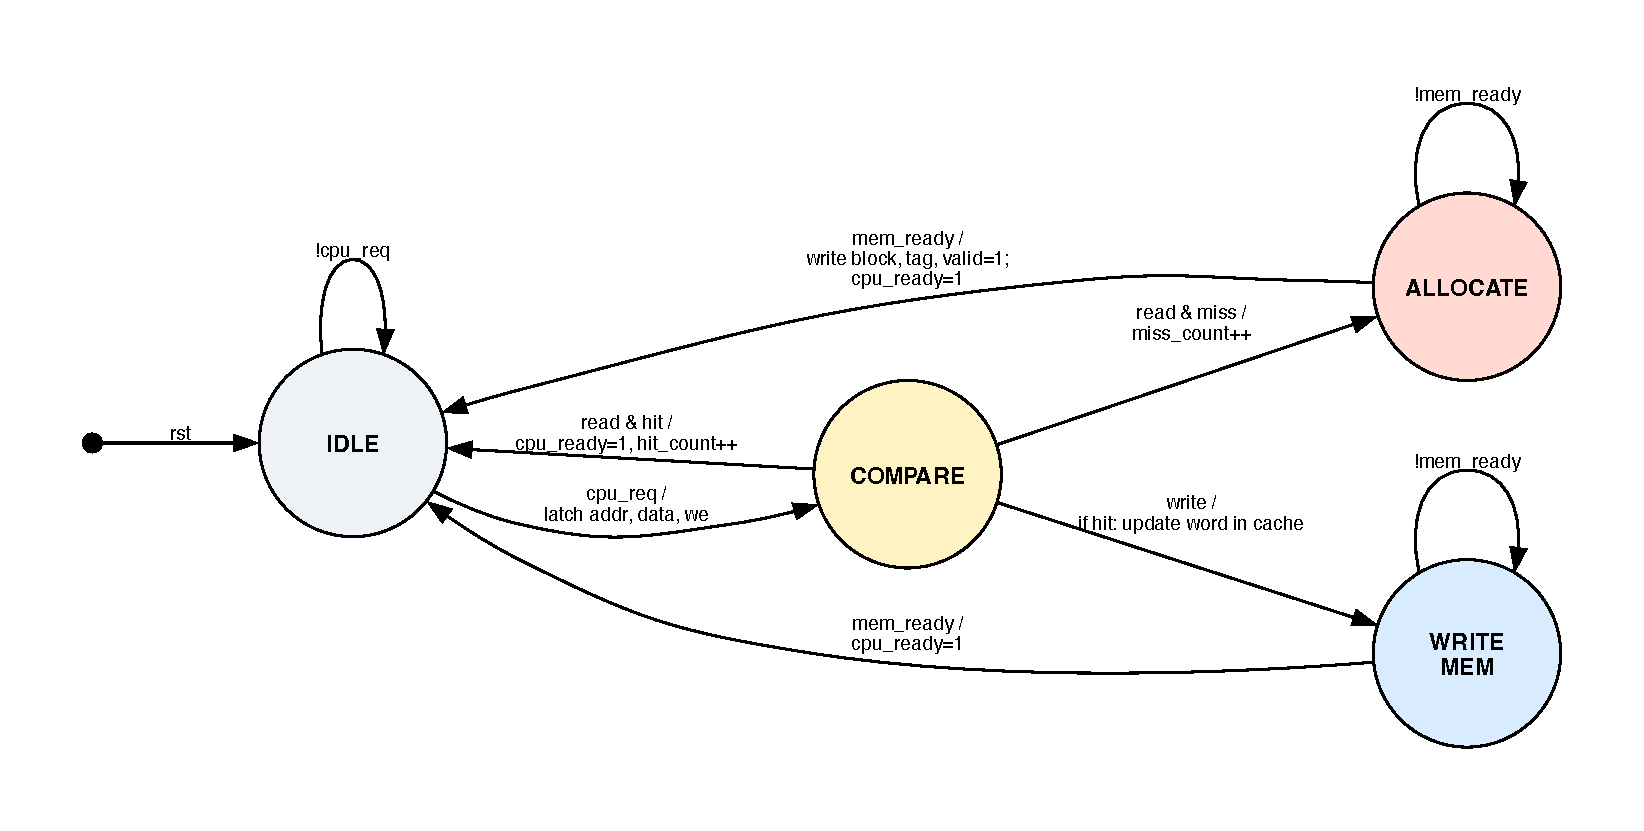
\includegraphics[width=\columnwidth]{../figures/fsm.pdf}
\caption{Cache controller state-transition diagram (condition / action).}
\label{fig:fsm}
\end{figure}

\subsection{RTL Module Hierarchy}
\begin{itemize}
\item \texttt{addr\_decoder.v}: tag / index / word-select extraction.
\item \texttt{cache\_rams.v}: \texttt{cache\_data\_ram} (supports a full-block refill or a single-word write), \texttt{cache\_tag\_ram}, \texttt{valid\_ram}.
\item \texttt{tag\_comparator.v}: valid-qualified equality compare.
\item \texttt{cache\_controller.v}: FSM, request latches, hit/miss counters.
\item \texttt{dm\_cache.v}: synthesizable top level that connects the modules above.
\item \texttt{main\_memory.v}: behavioral DRAM model with latency $L$ and a 128-bit block read (simulation only).
\end{itemize}

\subsection{Verification Methodology}
The testbench (\texttt{tb\_dm\_cache.v}) contains a \emph{golden reference model}: shadow valid/tag arrays plus a shadow copy of memory. For every access, the model predicts whether it should hit and what data it should return, then compares both with the DUT. At the end of each trace it also compares the totals with the hardware counters. The cache is reset (made cold) before each of six traces:
\begin{enumerate}
\item \textbf{Directed} (11 accesses): cold miss, temporal hit, spatial hits, write hit with read-back, write miss (checking no-allocate), conflict eviction, and a check that the writes reached main memory.
\item \textbf{Sequential}: 512 consecutive words (2\,KB).
\item \textbf{Repeated}: a 512-byte array read 4 times.
\item \textbf{Random}: 512 LFSR-generated word addresses in an 8\,KB window.
\item \textbf{Conflict}: two addresses 1\,KB apart (same index), alternated 64 times.
\item \textbf{Mixed R/W}: 512 random accesses in 2\,KB, about 3/8 of them writes.
\end{enumerate}
Simulation uses Icarus Verilog 12~\cite{icarus}. Every access is logged to \texttt{trace\_log.csv}, and the waveforms are dumped to VCD.

\subsection{Prototype Status and Preliminary Results}
All six traces pass with zero mismatches (Table~\ref{tab:results}). Fig.~\ref{fig:wave} shows the directed test. The first read of \texttt{0x1000} misses: the FSM goes COMPARE $\rightarrow$ ALLOCATE, \texttt{mem\_req} is held for 10 cycles, and \texttt{cpu\_ready} rises with \texttt{mem\_ready}, so the access takes 12 cycles. The next three reads to the same block hit in a single COMPARE cycle each, and \texttt{hit\_count} increments.

\begin{figure*}[t]
\centering
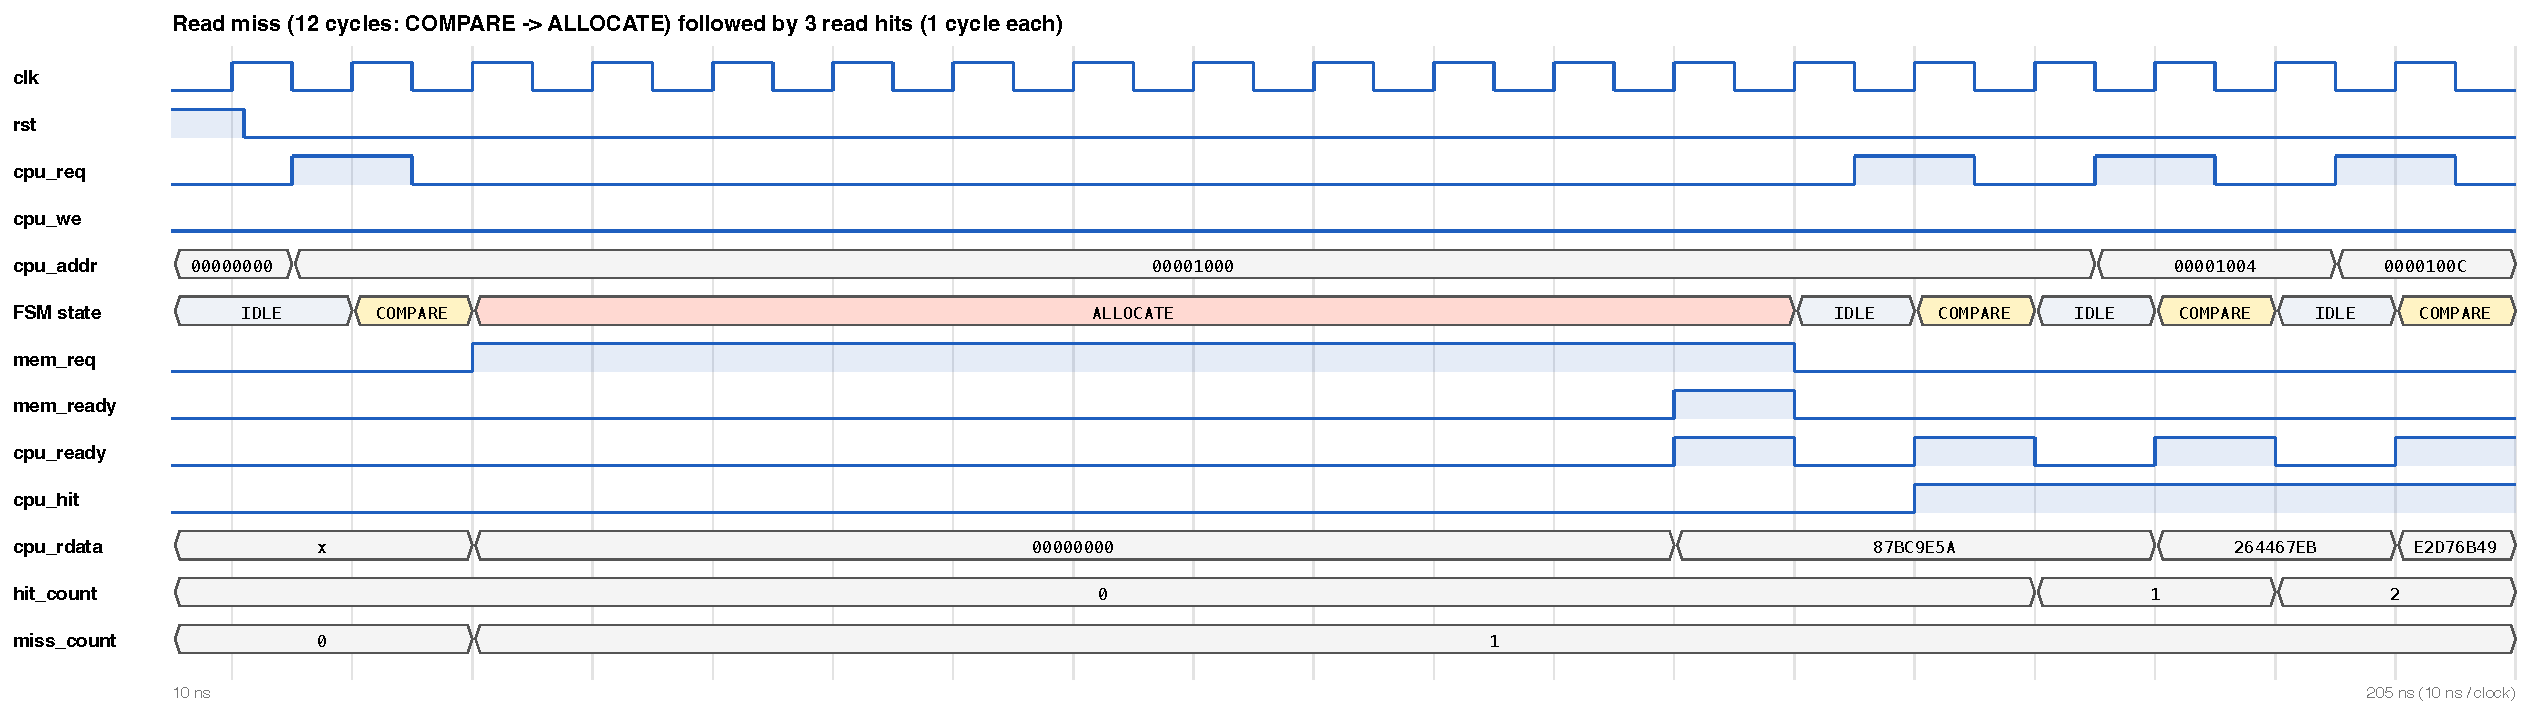
\includegraphics[width=\textwidth]{../figures/wave_miss_then_hits.pdf}
\caption{Simulation waveform: a 12-cycle read miss (refill from memory) followed by three 1-cycle read hits to the same block.}
\label{fig:wave}
\end{figure*}

\begin{table}[t]
\centering
\caption{Simulation results ($L=10$; AMAT over reads, in cycles)}
\label{tab:results}
\begin{tabular}{@{}lrrrrr@{}}
\toprule
Trace & Acc. & Hits & Hit \% & AMAT$_{meas}$ & AMAT$_{calc}$ \\ \midrule
Directed   & 11  & 6   & 54.55 & 5.89  & 5.89 \\
Sequential & 512 & 384 & 75.00 & 3.75  & 3.75 \\
Repeated   & 512 & 480 & 93.75 & 1.69  & 1.69 \\
Random     & 512 & 53  & 10.35 & 10.86 & 10.86 \\
Conflict   & 128 & 0   & 0.00  & 12.00 & 12.00 \\
Mixed R/W  & 512 & 217 & 42.38 & 7.19  & 7.19 \\ \bottomrule
\end{tabular}
\end{table}

The results match theory exactly:
\begin{itemize}
\item \textbf{Sequential}: one compulsory miss per 4-word block gives a 75\% hit rate. This is spatial locality, and the hit rate is bounded by the block size.
\item \textbf{Repeated}: only the 32 cold misses of the first pass occur ($1-32/512=93.75\%$). This is temporal locality, possible because the 512-byte array fits in the 1\,KB cache.
\item \textbf{Random}: an 8\,KB working set gives roughly the 1/8 hit rate expected from capacity.
\item \textbf{Conflict}: 0\% hits even though the cache is almost empty. This is the classic direct-mapped weakness~\cite{hill1989} and the motivation for the 2-way comparison in Phase~II.
\end{itemize}
The measured AMAT equals $1 + m \times 11$ to two decimal places, which validates the cycle-level timing of the controller.

\subsection{Phase II Plan}
\begin{enumerate}
\item Synthesize \texttt{dm\_cache} in Vivado and report LUT/FF/BRAM use and $F_{max}$.
\item Implement a 2-way set-associative LRU cache with the same interface and compare hit rate, AMAT and area on identical traces.
\item Sweep cache and block sizes and memory latency.
\item Add a write buffer to hide write-through latency, and compare write-through with write-back memory traffic.
\end{enumerate}

\section{Individual Contributions}
\begin{table}[h]
\centering
\caption{Work distribution}
\label{tab:contrib}
\begin{tabular}{@{}>{\raggedright\arraybackslash}p{0.27\columnwidth}>{\raggedright\arraybackslash}p{0.63\columnwidth}@{}}
\toprule
Member & Contribution \\ \midrule
\MemA & Controller FSM design and RTL (\texttt{cache\_controller}), hit/miss counters, state diagram; report: Proposed Solution (FSM). \\
\MemB & Cache storage: \texttt{cache\_data\_ram}, \texttt{cache\_tag\_ram}, \texttt{valid\_ram}; report: Literature Review. \\
\MemC & System architecture and address breakdown: \texttt{addr\_decoder}, \texttt{tag\_comparator}, block diagram; report: Introduction. \\
\MemD & \texttt{main\_memory} model, top-level integration (\texttt{dm\_cache}), waveform generation; report: Microarchitecture. \\
\MemE & Self-checking testbench, reference model, access traces, hit-rate/AMAT analysis; report: Results. \\ \bottomrule
\end{tabular}
\end{table}
All members reviewed the RTL, took part in the prototype video and maintain the GitHub repository (\url{\RepoURL}). Demo video: \url{\VideoURL}.

\section*{Conclusion (Phase I)}
We have built a working, fully verified direct-mapped cache controller prototype. Its measured hit rates and AMAT agree exactly with analytical predictions across sequential, repeated, random and conflicting access patterns.

\begin{thebibliography}{99}
\bibitem{wilkes1965} M.~V. Wilkes, ``Slave memories and dynamic storage allocation,'' \emph{IEEE Trans. Electron. Comput.}, vol.~EC-14, no.~2, pp.~270--271, Apr. 1965.
\bibitem{smith1982} A.~J. Smith, ``Cache memories,'' \emph{ACM Comput. Surv.}, vol.~14, no.~3, pp.~473--530, Sep. 1982.
\bibitem{hill1988} M.~D. Hill, ``A case for direct-mapped caches,'' \emph{Computer}, vol.~21, no.~12, pp.~25--40, Dec. 1988.
\bibitem{hill1989} M.~D. Hill and A.~J. Smith, ``Evaluating associativity in CPU caches,'' \emph{IEEE Trans. Comput.}, vol.~38, no.~12, pp.~1612--1630, Dec. 1989.
\bibitem{jouppi1990} N.~P. Jouppi, ``Improving direct-mapped cache performance by the addition of a small fully-associative cache and prefetch buffers,'' in \emph{Proc. 17th Annu. Int. Symp. Comput. Archit. (ISCA)}, 1990, pp.~364--373.
\bibitem{belady1966} L.~A. Belady, ``A study of replacement algorithms for a virtual-storage computer,'' \emph{IBM Syst. J.}, vol.~5, no.~2, pp.~78--101, 1966.
\bibitem{wulf1995} W.~A. Wulf and S.~A. McKee, ``Hitting the memory wall: Implications of the obvious,'' \emph{ACM SIGARCH Comput. Archit. News}, vol.~23, no.~1, pp.~20--24, Mar. 1995.
\bibitem{hp_coa} D.~A. Patterson and J.~L. Hennessy, \emph{Computer Organization and Design: The Hardware/Software Interface}, 5th~ed. Waltham, MA, USA: Morgan Kaufmann, 2014, ch.~5.
\bibitem{hp_caqa} J.~L. Hennessy and D.~A. Patterson, \emph{Computer Architecture: A Quantitative Approach}, 6th~ed. Cambridge, MA, USA: Morgan Kaufmann, 2017, ch.~2 and App.~B.
\bibitem{verilog2005} \emph{IEEE Standard for Verilog Hardware Description Language}, IEEE Std 1364-2005, 2006.
\bibitem{icarus} S.~Williams, ``Icarus Verilog,'' [Online]. Available: \url{https://steveicarus.github.io/iverilog/}
\end{thebibliography}
\end{document}
